%!TEX root = syntheyes15.tex

\section{Rendering photo-realistic training images}

We briefly describe how we use image-based lighting \cite{debevec2002image} to model a wide range of realistic lighting conditions, and finally discuss the details of our rendering setup.

\begin{figure}
    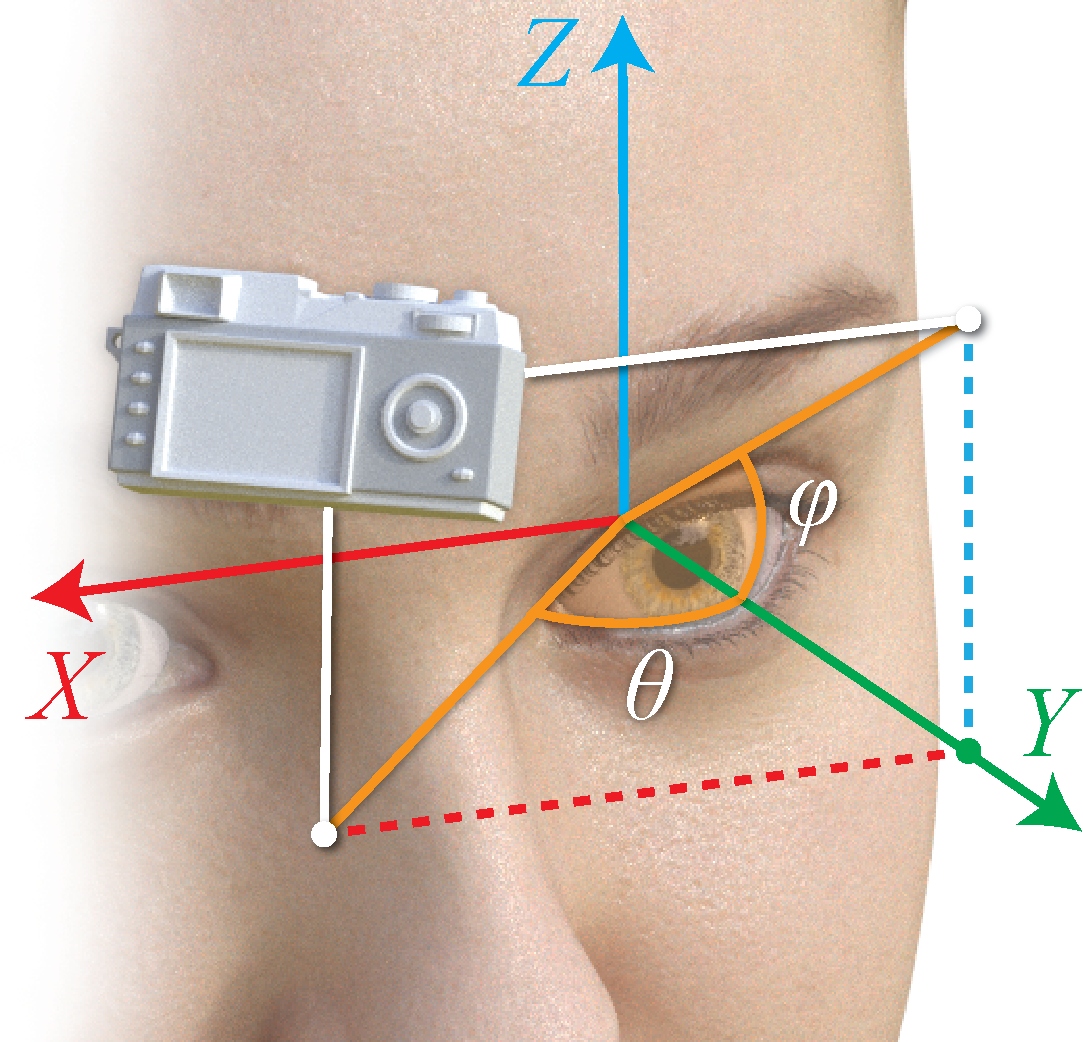
\includegraphics[width=0.4\columnwidth]{camera_position} \hfill
    \caption{How we position the camera.}
    \label{fig:participants}
\end{figure}

\subsection{Lighting}

\begin{figure}
    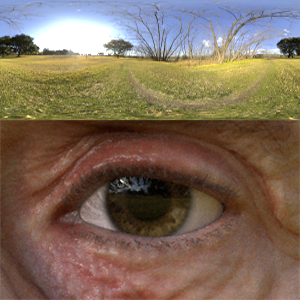
\includegraphics[width=0.24\columnwidth]{fig_env_1} \hfill
    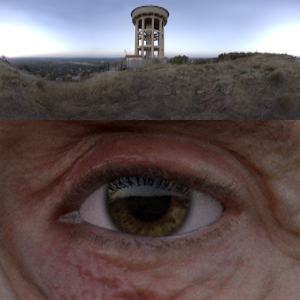
\includegraphics[width=0.24\columnwidth]{fig_env_2} \hfill
    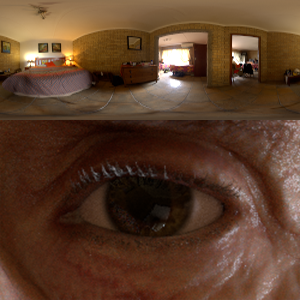
\includegraphics[width=0.24\columnwidth]{fig_env_3} \hfill
    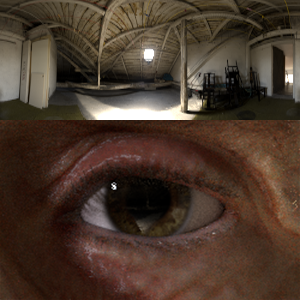
\includegraphics[width=0.24\columnwidth]{fig_env_4}
    \caption{Appearance variation from lighting is modelled with poseable high-dynamic-range environment maps \cite{debevec2002image}.}
    \label{fig:participants}
\end{figure}

\subsection{Computational setup}

We can rapidly generate diverse datasets much faster than manual collection and annotation.